\documentclass{ximera}

 

\usepackage{epsfig}

\graphicspath{
  {./}
  {figures/}
}

\usepackage{morewrites}
\makeatletter
\newcommand\subfile[1]{%
\renewcommand{\input}[1]{}%
\begingroup\skip@preamble\otherinput{#1}\endgroup\par\vspace{\topsep}
\let\input\otherinput}
\makeatother

\newcommand{\includeexercises}{\directlua{dofile("/home/jim/linearAlgebra/laode/exercises.lua")}}

%\newcounter{ccounter}
%\setcounter{ccounter}{1}
%\newcommand{\Chapter}[1]{\setcounter{chapter}{\arabic{ccounter}}\chapter{#1}\addtocounter{ccounter}{1}}

%\newcommand{\section}[1]{\section{#1}\setcounter{thm}{0}\setcounter{equation}{0}}

%\renewcommand{\theequation}{\arabic{chapter}.\arabic{section}.\arabic{equation}}
%\renewcommand{\thefigure}{\arabic{chapter}.\arabic{figure}}
%\renewcommand{\thetable}{\arabic{chapter}.\arabic{table}}

%\newcommand{\Sec}[2]{\section{#1}\markright{\arabic{ccounter}.\arabic{section}.#2}\setcounter{equation}{0}\setcounter{thm}{0}\setcounter{figure}{0}}

\newcommand{\Sec}[2]{\section{#1}}

\setcounter{secnumdepth}{2}
%\setcounter{secnumdepth}{1} 

%\newcounter{THM}
%\renewcommand{\theTHM}{\arabic{chapter}.\arabic{section}}

\newcommand{\trademark}{{R\!\!\!\!\!\bigcirc}}
%\newtheorem{exercise}{}

\newcommand{\dfield}{{\sf dfield9}}
\newcommand{\pplane}{{\sf pplane9}}

\newcommand{\EXER}{\section*{Exercises}}%\vspace*{0.2in}\hrule\small\setcounter{exercise}{0}}
\newcommand{\CEXER}{}%\vspace{0.08in}\begin{center}Computer Exercises\end{center}}
\newcommand{\TEXER}{} %\vspace{0.08in}\begin{center}Hand Exercises\end{center}}
\newcommand{\AEXER}{} %\vspace{0.08in}\begin{center}Hand Exercises\end{center}}

% BADBAD: \newcommand{\Bbb}{\bf}

\newcommand{\R}{\mbox{$\Bbb{R}$}}
\newcommand{\C}{\mbox{$\Bbb{C}$}}
\newcommand{\Z}{\mbox{$\Bbb{Z}$}}
\newcommand{\N}{\mbox{$\Bbb{N}$}}
\newcommand{\D}{\mbox{{\bf D}}}
\usepackage{amssymb}
%\newcommand{\qed}{\hfill\mbox{\raggedright$\square$} \vspace{1ex}}
%\newcommand{\proof}{\noindent {\bf Proof:} \hspace{0.1in}}

\newcommand{\setmin}{\;\mbox{--}\;}
\newcommand{\Matlab}{{M\small{AT\-LAB}} }
\newcommand{\Matlabp}{{M\small{AT\-LAB}}}
\newcommand{\computer}{\Matlab Instructions}
\newcommand{\half}{\mbox{$\frac{1}{2}$}}
\newcommand{\compose}{\raisebox{.15ex}{\mbox{{\scriptsize$\circ$}}}}
\newcommand{\AND}{\quad\mbox{and}\quad}
\newcommand{\vect}[2]{\left(\begin{array}{c} #1_1 \\ \vdots \\
 #1_{#2}\end{array}\right)}
\newcommand{\mattwo}[4]{\left(\begin{array}{rr} #1 & #2\\ #3
&#4\end{array}\right)}
\newcommand{\mattwoc}[4]{\left(\begin{array}{cc} #1 & #2\\ #3
&#4\end{array}\right)}
\newcommand{\vectwo}[2]{\left(\begin{array}{r} #1 \\ #2\end{array}\right)}
\newcommand{\vectwoc}[2]{\left(\begin{array}{c} #1 \\ #2\end{array}\right)}

\newcommand{\ignore}[1]{}


\newcommand{\inv}{^{-1}}
\newcommand{\CC}{{\cal C}}
\newcommand{\CCone}{\CC^1}
\newcommand{\Span}{{\rm span}}
\newcommand{\rank}{{\rm rank}}
\newcommand{\trace}{{\rm tr}}
\newcommand{\RE}{{\rm Re}}
\newcommand{\IM}{{\rm Im}}
\newcommand{\nulls}{{\rm null\;space}}

\newcommand{\dps}{\displaystyle}
\newcommand{\arraystart}{\renewcommand{\arraystretch}{1.8}}
\newcommand{\arrayfinish}{\renewcommand{\arraystretch}{1.2}}
\newcommand{\Start}[1]{\vspace{0.08in}\noindent {\bf Section~\ref{#1}}}
\newcommand{\exer}[1]{\noindent {\bf \ref{#1}}}
\newcommand{\ans}{}
\newcommand{\matthree}[9]{\left(\begin{array}{rrr} #1 & #2 & #3 \\ #4 & #5 & #6
\\ #7 & #8 & #9\end{array}\right)}
\newcommand{\cvectwo}[2]{\left(\begin{array}{c} #1 \\ #2\end{array}\right)}
\newcommand{\cmatthree}[9]{\left(\begin{array}{ccc} #1 & #2 & #3 \\ #4 & #5 &
#6 \\ #7 & #8 & #9\end{array}\right)}
\newcommand{\vecthree}[3]{\left(\begin{array}{r} #1 \\ #2 \\
#3\end{array}\right)}
\newcommand{\cvecthree}[3]{\left(\begin{array}{c} #1 \\ #2 \\
#3\end{array}\right)}
\newcommand{\cmattwo}[4]{\left(\begin{array}{cc} #1 & #2\\ #3
&#4\end{array}\right)}

\newcommand{\Matrix}[1]{\ensuremath{\left(\begin{array}{rrrrrrrrrrrrrrrrrr} #1 \end{array}\right)}}

\newcommand{\Matrixc}[1]{\ensuremath{\left(\begin{array}{cccccccccccc} #1 \end{array}\right)}}



\renewcommand{\labelenumi}{\theenumi)}
\newenvironment{enumeratea}%
{\begingroup
 \renewcommand{\theenumi}{\alph{enumi}}
 \renewcommand{\labelenumi}{(\theenumi)}
 \begin{enumerate}}
 {\end{enumerate}\endgroup}



\newcounter{help}
\renewcommand{\thehelp}{\thesection.\arabic{equation}}

%\newenvironment{equation*}%
%{\renewcommand\endequation{\eqno (\theequation)* $$}%
%   \begin{equation}}%
%   {\end{equation}\renewcommand\endequation{\eqno \@eqnnum
%$$\global\@ignoretrue}}

%\input{psfig.tex}

\author{Martin Golubitsky and Michael Dellnitz}

%\newenvironment{matlabEquation}%
%{\renewcommand\endequation{\eqno (\theequation*) $$}%
%   \begin{equation}}%
%   {\end{equation}\renewcommand\endequation{\eqno \@eqnnum
% $$\global\@ignoretrue}}

\newcommand{\soln}{\textbf{Solution:} }
\newcommand{\exercap}[1]{\centerline{Figure~\ref{#1}}}
\newcommand{\exercaptwo}[1]{\centerline{Figure~\ref{#1}a\hspace{2.1in}
Figure~\ref{#1}b}}
\newcommand{\exercapthree}[1]{\centerline{Figure~\ref{#1}a\hspace{1.2in}
Figure~\ref{#1}b\hspace{1.2in}Figure~\ref{#1}c}}
\newcommand{\para}{\hspace{0.4in}}

\renewenvironment{solution}{\suppress}{\endsuppress}

\ifxake
\newenvironment{matlabEquation}{\begin{equation}}{\end{equation}}
\else
\newenvironment{matlabEquation}%
{\let\oldtheequation\theequation\renewcommand{\theequation}{\oldtheequation*}\begin{equation}}%
  {\end{equation}\let\theequation\oldtheequation}
\fi

\makeatother


\title{Linearity}

\begin{document}
\begin{abstract}
\end{abstract}
\maketitle

  \label{S:linearity}

We begin by recalling the vector operations of addition and
scalar multiplication.  Given two $n$ vectors, vector addition
\index{vector!addition} is defined by
\[
\vect{x}{n}+\vect{y}{n}=\left(\begin{array}{c} x_1+y_1 \\ \vdots \\
x_n+y_n\end{array}\right).
\]
Multiplication of a scalar \index{scalar multiplication} times a vector
is defined by
\[
c\vect{x}{n} = \vect{cx}{n}.
\]
Using \eqref{Atimesx} we can check that matrix multiplication
satisfies
\begin{eqnarray}
A(x+y) & = & Ax + Ay \label{sum} \\
A(cx) & = & c(Ax). \label{product}
\end{eqnarray}
Using \Matlab we can also verify that the identities \eqref{sum}
and \eqref{product} are valid for some particular choices of $x$,
$y$, $c$ and $A$.  For example, let $c=5$ and
\begin{matlabEquation}\label{MATLAB:29}
A = \left(\begin{array}{cccc} 2 & 3 & 4 & 1\\ 1 & 1 & 2 & 3
\end{array}\right), \quad x = \left(\begin{array}{r} 1 \\ 5 \\ 4 \\
3 \end{array}\right), \quad y = \left(\begin{array}{r} 1 \\ -1 \\ -1 \\
4 \end{array}\right).
\end{matlabEquation}
Typing {\tt e3\_3\_3} enters this information into \Matlabp.  Now
type
\begin{verbatim}
z1 = A*(x+y)
z2 = A*x + A*y
\end{verbatim}
and compare {\tt z1} and {\tt z2}.  The fact that they are both
equal to
\[
\vectwo{35}{33}
\]
verifies \eqref{sum} in this case.  Similarly, type
\begin{verbatim}
w1 = A*(c*x)
w2 = c*(A*x)
\end{verbatim}
and compare {\tt w1} and {\tt w2} to verify \eqref{product}.


The central idea in linear algebra is the notion of
{\em linearity\/}. \index{linear}
\begin{definition} \label{linearity}
A mapping $L:\R^n\to\R^m$ is {\em linear}\index{linear!mapping}
if
\begin{itemize}
\item[(a)]  $L(x+y) = L(x) + L(y)$ for all $x,y\in\R^n$.
\item[(b)]  $L(cx) = cL(x)$ for all $x\in\R^n$ and all scalars
$c\in\R$.
\end{itemize}
\end{definition}

To better understand the meaning of Definition~\ref{linearity}(a,b),
we verify these conditions for the mapping $L:\R^2\to\R^2$ defined by
\begin{equation}  \label{E:mme}
L(x) = (x_1+3x_2,2x_1-x_2),
\end{equation}
where $x=(x_1,x_2)\in\R^2$.  To verify Definition~\ref{linearity}(a), let
$y=(y_1,y_2)\in\R^2$.  Then
\begin{eqnarray*}
L(x+y) & = & L(x_1+y_1,x_2+y_2)\\
& = & ((x_1+y_1)+3(x_2+y_2), 2(x_1+y_1)-(x_2+y_2)) \\
 & = & (x_1+y_1+3x_2+3y_2, 2x_1+2y_1-x_2-y_2).
\end{eqnarray*}
On the other hand,
\begin{eqnarray*}
L(x)+L(y) & = & (x_1+3x_2,2x_1-x_2) + (y_1+3y_2,2y_1-y_2) \\
 & = & (x_1+3x_2+y_1+3y_2, 2x_1-x_2+2y_1-y_2).
\end{eqnarray*}
Hence
\[
L(x+y) = L(x) + L(y)
\]
for every pair of vectors $x$ and $y $ in $\R^2$.

Similarly, to verify Definition~\ref{linearity}(b), let $c\in\R$ be a scalar
and compute
\[
L(cx) = L(cx_1,cx_2)=((cx_1)+3(cx_2),2(cx_1)-(cx_2)).
\]
Then compute
\[
cL(x) = c(x_1+3x_2,2x_1-x_2)= (c(x_1+3x_2), c(2x_1-x_2)),
\]
from which it follows that
\[
L(cx) = cL(x)
\]
for every vector $x\in\R^2$ and every scalar $c\in\R$.  Thus $L$ is a linear 
mapping.

In fact, the mapping \eqref{E:mme} is a matrix mapping and could
have been written in the form
\[
L(x) = \mattwo{1}{3}{2}{-1}x.
\]
Hence the linearity of $L$ could have been checked using identities
\eqref{sum} and \eqref{product}.  Indeed, matrix mappings are always linear
mappings, as we now discuss.

\subsubsection*{Matrix Mappings are Linear Mappings}

Let $A$ be an $m\times n$ matrix and recall that the matrix mapping
$L_A:\R^n\to\R^m$ is defined by $L_A(x)=Ax$.  We may rewrite \eqref{sum} and
\eqref{product} using this notation as
\begin{eqnarray*}
L_A(x+y) & = & L_A(x) + L_A(y) \\
L_A(cx) & = & cL_A(x).
\end{eqnarray*}
Thus all matrix mappings\index{matrix!mappings} are linear
mappings\index{linear!mapping}.  We will show that all linear
mappings are matrix mappings (see Theorem~\ref{lin-matrices}).  But first
we discuss linearity in the simplest context of mappings from $\R\to\R$.

\subsection*{Linear and Nonlinear Mappings of $\R\to\R$}

Note that $1\times 1$ matrices are just scalars $A=(a)$.  It follows from
\eqref{sum} and \eqref{product} that we have shown that the matrix mappings
$L_A(x)=ax$ are all linear, though this point could have been verified
directly.  Before showing that these are all the linear mappings of
$\R\to\R$, we focus on examples of functions of $\R\to\R$ that are
{\em not\/} linear.

\subsubsection*{Examples of Mappings that are Not Linear}

\begin{itemize}
\item   $f(x)=x^2$.  Calculate
\[
f(x+y) = (x+y)^2 = x^2+2xy+y^2
\]
while
\[
f(x)+f(y) = x^2 + y^2.
\]
The two expressions are not equal and $f(x)=x^2$ is not linear.
\item   $f(x)=e^x$.  Calculate
\[
f(x+y) = e^{x+y} = e^x e^y
\]
while
\[
f(x)+f(y) = e^x + e^y.
\]
The two expressions are not equal and $f(x)=e^x$ is not linear.
\item   $f(x) = \sin x$.  Recall that
\[
f(x+y) =\sin(x+y) = \sin x \cos y +\cos x \sin y
\]
while
\[
f(x)+f(y) = \sin x + \sin y.
\]
The two expressions are not equal and $f(x)=\sin x $ is not
linear.
\end{itemize}

\subsubsection*{Linear Functions of One Variable}

Suppose we take the opposite approach and ask what functions of
$\R\to\R$ are linear.  Observe that if $L:\R\to\R$ is linear,
then
\[
L(x) = L(x\cdot 1).
\]
Since we are looking at the special case of linear mappings on
$\R$, we note that $x$ is a real number as well as a vector.
Thus we can use Definition~\ref{linearity}(b) to observe that
\[
L(x\cdot 1)=xL(1).
\]
So if we let $a=L(1)$, then we see that
\[
L(x)=ax.
\]
Thus linear mappings of $\R$ into $\R$ are very special mappings
indeed; they are all scalar multiples of the identity mapping.

\subsection*{All Linear Mappings are Matrix Mappings}

We end this section by proving that every linear mapping is
given by matrix multiplication. But first we state and prove two
lemmas.  There is a standard set of vectors that is used over
and over again in linear algebra, which we now define.

\begin{definition}  \label{D:canonicalbasis}
Let $j$ be an integer between $1$ and $n$.  The $n$-vector $e_j$ is
the vector that has a $1$ in the $j^{th}$ entry and zeros in all
other entries.
\end{definition} \index{$e_j$}

\begin{lemma}  \label{linequal}
Let $L_1:\R^n\to\R^m$ and $L_2:\R^n\to\R^m$ be linear mappings.
Suppose that $L_1(e_j)=L_2(e_j)$ for every $j=1,\ldots,n$.  Then
$L_1=L_2$.
\end{lemma}

\begin{proof}  Let $x=(x_1,\ldots,x_n)$ be a vector in $\R^n$.  Then
\[
x = x_1e_1 + \cdots + x_ne_n.
\]
Linearity of $L_1$ and $L_2$ implies that
\begin{eqnarray*}
L_1(x) & = & x_1L_1(e_1) + \cdots + x_nL_1(e_n) \\
  & = & x_1L_2(e_1) + \cdots + x_nL_2(e_n) \\
  & = & L_2(x).
\end{eqnarray*}
Since $L_1(x)=L_2(x)$ for all $x\in\R^n$, it follows that
$L_1=L_2$.  \end{proof}

\begin{lemma}  \label{columnsA}
Let $A$ be an $m\times n$ matrix.  Then $Ae_j$ is the $j^{th}$
column of $A$.
\end{lemma}

\begin{proof}  Recall the definition of matrix multiplication given in \eqref{Atimesx}.
In that formula, just set $x_i$ equal to zero for all $i\neq j$ and set
$x_j=1$. \end{proof}

\begin{theorem}  \label{lin-matrices}
Let $L:\R^n\to\R^m$ be a linear mapping\index{linear!mapping}.
Then there exists an $m\times n$ matrix $A$ such that $L=L_A$.
\end{theorem}

\begin{proof}
There are two steps to the proof: determine the matrix $A$ and
verify that $L_A=L$.

Let $A$ be the matrix whose $j^{th}$ column is $L(e_j)$.  By
Lemma~\ref{columnsA} $L(e_j) = Ae_j$; that is, $L(e_j) = L_A(e_j)$.
Lemma~\ref{linequal} implies that $L=L_A$.  \end{proof}

Theorem~\ref{lin-matrices} provides a simple way of showing that
\[
L(0) = 0
\]
for any linear map $L$.  Indeed, $L(0)=L_A(0)=A0=0$ for some matrix $A$.  
(This fact can also be proved directly from the definition of linear mapping.)

\subsubsection*{Using Theorem~\protect\ref{lin-matrices} to Find Matrices
Associated to Linear Maps}

The proof of Theorem~\ref{lin-matrices} shows that the $j^{th}$ column of the
matrix $A$ associated to a linear mapping $L$ is $L(e_j)$ viewed as a column
vector.  As an example, let $L:\R^2\to\R^2$ be rotation clockwise through
$90^\circ$.  Geometrically, it is easy to see that
\[
  L(e_1) = L\left(\vectwo{1}{0}\right) = \vectwo{0}{-1}
\]
and
\[
L(e_2) = L\left(\vectwo{0}{1}\right) = \vectwo{1}{0}.
\]
Since we know that rotations are linear maps, it follows that the matrix
$A$ associated to the linear map $L$ is:
\[
A = \mattwo{0}{1}{-1}{0}.
\]
Additional examples of linear mappings whose associated matrices can be found
using Theorem~\ref{lin-matrices} are given in Exercises \ref{c4.3.7} --
\ref{c4.3.10}.



\EXER

\TEXER

\begin{exercise} \label{c4.3.1}
Compute $ax+by$ for each of the following:
\begin{itemize}
\item[(a)] $a=2$, $b=-3$, $x=(2,4)$ and $y=(3,-1)$.
\item[(b)] $a=10$, $b=-2$, $x=(1,0,-1)$ and $y=(2,-4,3)$.
\item[(c)] $a=5$, $b=-1$, $x=(4,2,-1,1)$ and $y=(-1,3,5,7)$.
\end{itemize}

\begin{solution}

(a) $2(2,4) - 3(3,-1) = (-5,11)$;

(b) $10(1,0,-1) - 2(2,-4,3) = (6,8,-16)$;

(c) $5(4,2,-1,1) - 1(-1,3,5,7) = (21,7,-10,-2)$.

\end{solution}
\end{exercise}

\begin{exercise} \label{c4.3.2}
Let $x=(4,7)$ and $y=(2,-1)$.  Write the vector $\alpha x+\beta
y$ as a vector in coordinates.

\begin{solution}

$\alpha (4,7) + \beta (2,-1) = (4\alpha + 2\beta, 7\alpha - \beta)$.

\end{solution}
\end{exercise}

\begin{exercise} \label{c4.3.3}
Let $x=(1,2)$, $y=(1,-3)$, and $z=(-2,-1)$.  Show that you can
write
\[
z=\alpha x+ \beta y
\]
for some $\alpha,\beta\in\R$.

\noindent {\bf Hint:} Set up a system of two linear equations in
the unknowns $\alpha$ and $\beta$, and then solve this linear
system.

\begin{solution}

The equation
\[ (-2, -1) = \alpha(1,2) + \beta(1,-3) =
(\alpha + \beta, 2\alpha - 3\beta ) \]
can be rewritten as the linear system
\[ \begin{array}{rrrrr}
-2 & = & \alpha & + & \beta \\
-1 & = & 2\alpha & - & 3\beta\end{array}. \]
Solving this system yields $\alpha = -\frac{7}{5}$ and
$\beta = -\frac{3}{5}$.

\end{solution}
\end{exercise}

\begin{exercise} \label{c4.3.4}
Can the vector $z=(2,3,-1)$ be written as
\[
z=\alpha x+ \beta y
\]
where $x=(2,3,0)$ and $y=(1,-1,1)$?

\begin{solution}

\ans The vector $z = (2,3,-1)$ cannot be written as
\[
z = \alpha(2,3,0) + \beta(1,-1,1).
\]

\soln Write the equation
\[ (2,3,-1) = \alpha(2,3,0) + \beta(1,-1,1) = 
(2\alpha + \beta, 3\alpha - \beta, \beta) \]
as a linear system of two unknowns in three equations:
\[ \begin{array}{rrrrr}
2 & = & 2\alpha & + & \beta \\
3 & = & 3\alpha & - & \beta \\
-1 & = & \beta \end{array}. \]
Substituting $\beta = -1$ into the first and second equations
yields
\[ \begin{array}{rcl}
\frac{3}{2} & = & \alpha \\
\frac{2}{3} & = & \alpha. \end{array} \]
The system is inconsistent, so there is no solution to the desired
equation.

\end{solution}
\end{exercise}

\begin{exercise} \label{c4.3.5}
Let $x=(3,-2)$, $y=(2,3)$, and $z=(1,4)$.  For which real
numbers $\alpha,\beta,\gamma$ does
\[
\alpha x + \beta y + \gamma z = (1,-2)?
\]

\begin{solution}

\ans The equation
\[ \alpha(3,-2) + \beta(2,3) + \gamma(1,4) = (1,-2) \]
holds for any real numbers $\alpha$,$\beta$,
$\gamma$ such that $\alpha = \frac{5}{13}\gamma +
\frac{7}{13}$ and $\beta = -\frac{14}{13}\gamma
- \frac{4}{13}$.

\soln Write the equation as the linear system
\[ \begin{array}{rrrrrrl}
3\alpha & + & 2\beta & + & \gamma & = & 1 \\
-2\alpha & + & 3\beta & + & 4\gamma & = & -2. \end{array} \]
The augmented matrix
\[ \left(\begin{array}{rrr|r}
3 & 2 & 1 & 1 \\
-2 & 3 & 4 & -2 \end{array}\right) \]
row reduces to
\[ \left(\begin{array}{rrr|r}
1 & 0 & -\frac{5}{13} & \frac{7}{13} \\
0 & 1 & \frac{14}{13} & -\frac{4}{13} \end{array}\right) \]
and the equation is valid for any values of $\alpha$,$\beta$,
and $\gamma$ that satisfy this system.

\end{solution}
\end{exercise}

\noindent In Exercises~\ref{c4.3.6a} -- \ref{c4.3.6d} determine
whether the given transformation is linear.
\begin{exercise} \label{c4.3.6a}
  $T:\R^3\to\R^2$ defined by $T(x_1,x_2,x_3)=(x_1+2x_2-x_3,x_1-4x_3)$.

\begin{solution}
\ans The transformation $T(x,y,z) = (x + 2y - z, x - 4z)$
is linear.

\soln Use the definition that a mapping is linear if it satisfies
\eqref{sum} and \eqref{product} to verify:

\para Let $X_1 = (x_1,y_1,z_1)$ and let $X_2 = (x_2,y_2,z_2)$.
Verify \eqref{sum} by computing $T(X_1 + X_2)$ and comparing it
to $T(X_1) + T(X_2)$.
\[ \begin{array}{rcl}
T(X_1 + X_2) & = & T((x_1,y_1,z_1) + (x_2, y_2, z_2)) \\
& = & T(x_1 + x_2, y_1 + y_2, z_1 + z_2) \\
& = & ((x_1 + x_2) + 2(y_1 + y_2) - (z_1 + z_2),
(x_1 + x_2) - 4(z_1 + z_2)) \\ & = &
(x_1 + x_2 + 2y_1 + 2y_2 - z_1 - z_2, x_1 + x_2 - 4z_1 - 4z_2) \\
& = & (x_1 + 2y_1 - z_1, x_1 - 4z_1) +
(x_2 + 2y_2 - z_2, x_2 - 4z_2). \end{array} \]
\[ \begin{array}{rcl}
T(X_1) + T(X_2)
& = & T(x_1,y_1,z_1) + T(x_2,y_2,z_2) \\
& = & (x_1 + 2y_1 - z_1, x_1 - 4z_1) +
(x_2 + 2y_2 - z_2, x_2 - 4z_2). \end{array} \]
Let $X = (x,y,z)$ and let $c$ be any real scalar.  Verify
\eqref{product} by computing $cT(X)$ and comparing it to $T(cX)$.
\[ \begin{array}{rcl}
cT(X) & = & cT(x,y,z) \\
& = & c(x + 2y - z, x - 4z) \\
& = & (cx + 2cy - cz, cx - 4cz). \end{array} \]
\[ \begin{array}{rcl}
T(cX) & = & T(cx,cy,cz) \\
& = & T(cX) \\
& = & (cx + 2cy - cz, cx - 4cz). \end{array} \]
So $T(x,y,z) = (x + 2y - z, x - 4z)$ is a linear mapping.

\end{solution}
\end{exercise}
\begin{exercise} \label{c4.3.6b}
  $T:\R^2\to\R^2$ defined by $T(x_1,x_2)=(x_1+x_1x_2,2x_2)$.

\begin{solution}
\ans The transformation $T(x,y) = (x + xy, 2y)$ is not linear.

\soln If $T$ is a linear transformation, then
\[
T(x_1 + x_2,y_1 + y_2) = T(x_1,y_1) + T(x_2,y_2)
\]
for any real numbers $x_1$,$x_2$,$y_1$,$y_2$.  However,
\[
\begin{array}{rcl}
T(1,1) & = & (2,2) \\
T(1,0) + T(0,1) & = & (1,0) + (0,2) = (1,2).\end{array}
\]
Therefore $T(1,1) \neq T(1,0) + T(0,1)$ and $T$ is not linear.

\end{solution}
\end{exercise}
\begin{exercise} \label{c4.3.6c}
  $T:\R^2\to\R^2$ defined by $T(x_1,x_2)=(x_1+x_2,x_1-x_2-1)$.

\begin{solution}
The transformation $T(x,y) = (x + y, x - y - 1)$
is not linear because $T(0,0) = (0,-1) \neq 0$, contradicting
Theorem~\ref{lin-matrices}.

\end{solution}
\end{exercise}
\begin{exercise} \label{c4.3.6d}
  $T:\R^2\to\R^3$ defined by $T(x_1,x_2)=(1,x_1+x_2,2x_2)$

\begin{solution}
The transformation $T(x,y) = (1,x + y, 2y)$ is not linear
because $T(0,0) = (1,0,0) \neq 0$.

\end{solution}
\end{exercise}

\begin{exercise} \label{c4.3.7}
Find the $2\times 3$ matrix $A$ that satisfies
\[
Ae_1  =  \vectwo{2}{3},\qquad
Ae_2  =  \vectwo{1}{-1}, \AND
Ae_3  = \vectwo{0}{1}.
\]

\begin{solution}

\ans The matrix that satisfies these conditions is
\[
A = \left(\begin{array}{rrr} 2 & 1 & 0 \\ 3 & -1 & 1
\end{array}\right).
\]

\soln Let
\[
A = \left(\begin{array}{rrr}
a_{11} & a_{12} & a_{13} \\ a_{21} & a_{22} & a_{23}
\end{array}\right).
\]
Rewrite the conditions on $A$ as:
\[
\left(\begin{array}{rrr}
a_{11} & a_{12} & a_{13} \\ a_{21} & a_{22} & a_{23}
\end{array}\right) \vecthree{1}{0}{0} = \vectwo{2}{3}
\]
\[
\left(\begin{array}{rrr}
a_{11} & a_{12} & a_{13} \\ a_{21} & a_{22} & a_{23}
\end{array}\right) \vecthree{0}{1}{0} = \vectwo{1}{-1}
\]
\[
\left(\begin{array}{rrr}
a_{11} & a_{12} & a_{13} \\ a_{21} & a_{22} & a_{23}
\end{array}\right) \vecthree{0}{0}{1} = \vectwo{0}{1}
\]
These equations imply:
\[ \begin{array}{rcl} a_{11} & = & 2 \\ a_{21} & = & 3 \end{array},
\quad
\begin{array}{rcr} a_{12} & = & 1 \\ a_{22} & = & -1 \end{array}
\AND
\begin{array}{rcl} a_{13} & = & 0 \\ a_{23} & = & 1 \end{array}
\]
and determine the matrix $A$.

\end{solution}
\end{exercise}

\begin{exercise} \label{c4.3.8}
The {\em cross product\/} of two $3$-vectors $x=(x_1,x_2,x_3)$
and $y=(y_1,y_2,y_3)$ is the $3$-vector
\[
x\times y = (x_2y_3-x_3y_2,-(x_1y_3-x_3y_1),x_1y_2-x_2y_1).
\]
Let $K=(2,1,-1)$.  Show that the mapping $L:\R^3\to\R^3$ defined by
\[
L(x) = x\times K
\]
is a linear mapping.  Find the $3\times 3$ matrix $A$ such that
\[
L(x) = Ax,
\]
that is, $L=L_A$.

\begin{solution}

\ans The matrix of linear mapping $L$ is
\[
A = \matthree{0}{-1}{-1}{1}{0}{2}{1}{-2}{0}.
\]

\soln Let $X = (x_1,x_2,x_3)$ and let $Y = (y_1,y_2,y_3)$.  
Since $K = (2,1,-1)$,
\[
L(X) = (x_1,x_2,x_3) \times K = 
(-x_2 - x_3, x_1 + 2x_3, x_1 - 2x_2).
\]

To show that $L(X)$ is a linear mapping, first demonstrate that
\eqref{sum} is valid:
\[
\begin{array}{rcl}
L(X + Y) & = & L(x_1 + y_1,x_2 + y_2,x_3 + y_3) \\
& = & (-(x_2 + y_2) - (x_3 + y_3), (x_1 + y_1) + 2(x_3 + y_3),
(x_1 + y_1) - 2(x_2 + y_2)) \\
& = & (-x_2 - x_3, x_1 + 2x_3, x_1 - 2x_2) +
(-y_2 - y_3, y_1 + 2y_3, y_1 - 2y_2) \\
& = & L(X) + L(Y), \end{array}
\]
then show that \eqref{product} is valid:
\[
\begin{array}{rcl}
cL(X) & = & cL(x_1,x_2,x_3) \\
& = & c(-x_2 - x_3, x_1 + 2x_3, x_1 - 2x_2) \\
& = & (-cx_2 - cx_3, cx_1 + 2cx_3, cx_1 - 2cx_2) \\
& = & L(cx_1,cx_2,cx_3) \\
& = & L(cX). \end{array}
\]

Find $A$ by noting that $L(e_j) = Ae_j$ is the $j^{th}$ column of $A$,
and computing
\[ \begin{array}{l}
L(e_1) = L(1,0,0) = (0,1,1) \\
L(e_2) = L(0,1,0) = (-1,0,-2) \\
L(e_3) = L(0,0,1) = (-1,2,0). \end{array} \]


\end{solution}
\end{exercise}

\begin{exercise} \label{c4.3.9}
Argue geometrically that rotation of the plane counterclockwise
through an angle of $45^\circ$ is a linear mapping.  Find a
$2\times 2$ matrix $A$ such that $L_A$ rotates the plane
counterclockwise by $45^\circ$.

\begin{solution}

To see that $L(X + Y) = L(X) + L(Y)$, consider $X$ and $Y$ as
vectors.  These vectors are two sides of a parallelogram with
diagonal $X + Y$, as shown in Figure~\ref{c4.3.9}a.  Rotating
the plane $45^\circ$ counterclockwise has the effect of
rotating the entire parallelogram, as in Figure~\ref{c4.3.9}b.
Therefore, adding $X$ and $Y$ and then rotating the sum
$X + Y$ is the same as rotating $X$ and $Y$ separately and
then adding them.

\para To see that $cL(X) = L(cX)$, note that multiplying a
vector $X$ by a scalar $c$ affects only the length of the vector,
and that rotating the plane affects only the orientation of
the vector.  Therefore, the two operations can be performed in
either order with the same effect.

\para To find the matrix $A$ of this transformation, we can use
\eqref{e:rotmat}:
\[ A = \mattwo{\cos 45^\circ}{-\sin 45^\circ}{\sin 45^\circ}{\cos 45^\circ}
= \mattwo{\frac{1}{\sqrt{2}}}{-\frac{1}{\sqrt{2}}}
{\frac{1}{\sqrt{2}}}{\frac{1}{\sqrt{2}}} \]

\begin{figure}[htb]
                       \centerline{%
                       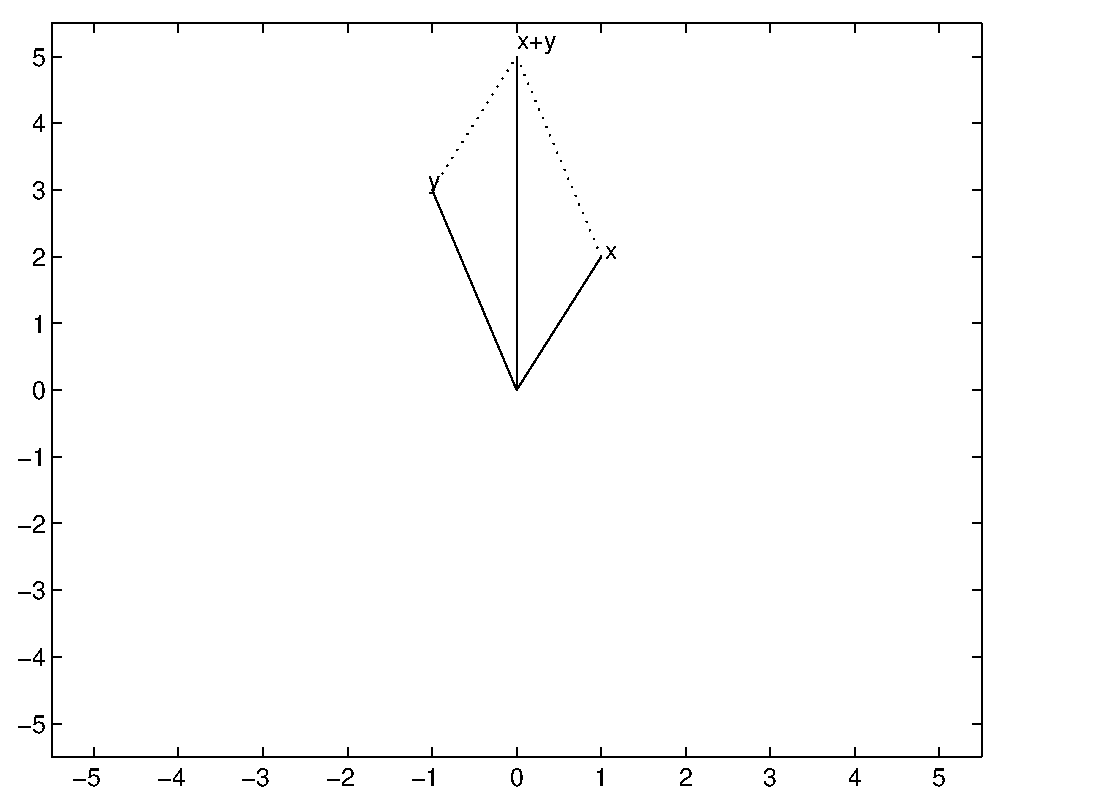
\psfig{file=exfigure/4-3-9a.eps,width=2.75in}
                       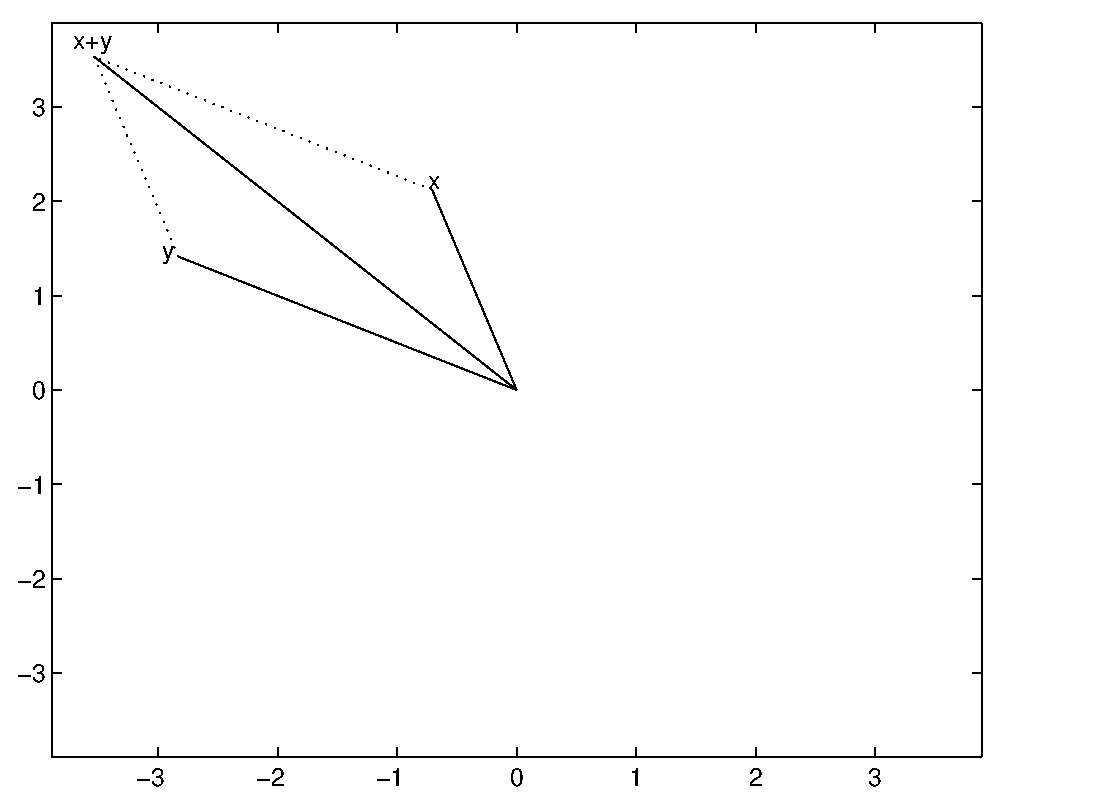
\psfig{file=exfigure/4-3-9b.eps,width=2.75in}}
                \exercaptwo{c4.3.9}
\end{figure}

\end{solution}
\end{exercise}

\begin{exercise} \label{c4.3.10}
Let $\sigma$ permute coordinates cyclically in $\R^3$; that is,
\[
\sigma(x_1,x_2,x_3) = (x_2,x_3,x_1).
\]
Find a $3\times 3$ matrix $A$ such that $\sigma = L_A$.

\begin{solution}

\ans The matrix of linear mapping $L_A$ is
\[ A = \matthree{0}{1}{0}{0}{0}{1}{1}{0}{0}. \]

\soln Note that if $\sigma = L_A$, then $\sigma(e_j) = Ae_j$ is the
$j^{th}$ column of matrix $A$.  Thus $A$ is determined by
\[
\begin{array}{l}
\sigma(e_1) = \sigma(1,0,0) = (0,0,1) \\
\sigma(e_2) = \sigma(0,1,0) = (1,0,0) \\
\sigma(e_3) = \sigma(0,0,1) = (0,1,0). \end{array}
\]


\end{solution}
\end{exercise}

\begin{exercise} \label{c4.3.11}
Let $L$ be a linear map.  Using the definition of linearity,
prove that $L(0)=0$.

\begin{solution}

Let $L(0) = K$.
By the definition of linearity, for any real number $c$,
\[ L(0) = L(c0) = cL(0) \]
which is valid only when $L(0) = 0$.

\end{solution}
\end{exercise}

\begin{exercise}  \label{c4.3.12}
Let $P:\R^n\to\R^m$ and $Q:\R^n\to\R^m$ be linear mappings. Prove
that $S:\R^n\to\R^m$ defined by
\[
S(x) = P(x) + Q(x)
\]
is also a linear mapping.  Theorem~\ref{lin-matrices} states that there
are matrices $A$, $B$ and $C$ such that
\[
P = L_A \AND Q = L_B \AND S = L_C .
\]
What is the relationship between the matrices $A$, $B$, and $C$?

\begin{solution}

The mapping $L(x)$ is linear if $L(x + y) = L(x) + L(y)$ and
if $cL(x) = L(cx)$.  We can use the assumption that $L_1(x)$
and $L_2(x)$ are linear mappings to show:
\[ \begin{array}{rcl}
L(x + y) & = & L_1(x + y) + L_2(x + y) \\
& = & L_1(x) + L_1(y) + L_2(x) + L_2(y) \\
& = & [L_1(x) + L_2(x)] + [L_1(y) + L_2(y)] \\
& = & L(x) + L(y) \end{array} \]
and
\[ \begin{array}{rcl}
cL(x) & = & cL_1(x) + cL_2(x) \\
& = & L_1(cx) + L_2(cx) \\
& = & L(cx). \end{array} \]

Assume that $L = L_A$, $L_1 = L_{A_1}$ and $L_2 = L_{A_2}$ for
$m \times n$ matrices $A$, $A_1$, $A_2$.  We claim that
$A = A_1 + A_2$, where $A_1 + A_2$ is the matrix obtained by
adding corresponding entries of $A_1$ and $A_2$.  By
definition, $L(e_j) = L_1(e_j) + L_2(e_j)$.  Lemma~\ref{columnsA}
implies that the $j^{th}$ column of $A$ is the sum of the
$j^{th}$ columns of $A_1$ and $A_2$ for all columns {j}, so
$A = A_1 + A_2$.

\end{solution}
\end{exercise}

\CEXER

\begin{exercise} \label{c4.3.13}
Let
\[
A = \mattwo{0.5}{0}{0}{2}.
\]
Use {\sf map} to verify that the linear mapping $L_A$ halves
the $x$-component of a point while it doubles the $y$-component.

\begin{solution}
Computer experiment.

\end{solution}
\end{exercise}

\begin{exercise} \label{c4.3.14}
Let
\[
A = \mattwo{0}{0.5}{-0.5}{0}.
\]
Use {\sf map} to determine how the mapping $L_A$ acts on $2$-vectors.
Describe this action in words.

\begin{solution}

The mapping $L_A$ performs the transformation $(x,y) \rightarrow
(0.5y, -0.5x)$.  That is, the mapping rotates a 2-vector
$90^\circ$ clockwise then halves its length.

\end{solution}
\end{exercise}

\noindent In Exercises~\ref{c4.3.15A} -- \ref{c4.3.15B} use \Matlab to
verify \eqref{sum} and \eqref{product}.
\begin{exercise} \label{c4.3.15A}
\begin{matlabEquation} \label{eq4.3.15a}
A = \left(
\begin{array}{rrr}
 1 & 2 & 3  \\
 0 & 1 & -2  \\
 4 & 0 & 1
\end{array}
\right),\quad
x=\left(
\begin{array}{r}
 3   \\
 2   \\
 -1
\end{array}
\right),\quad
y=\left(
\begin{array}{r}
 0   \\
 -5   \\
 10
\end{array}
\right),\quad c=21;
\end{matlabEquation}

\begin{solution}
Verify \eqref{sum} by typing {\tt A*(x + y)} to obtain:
\begin{verbatim}
ans =
    24
   -21
    21
\end{verbatim}
Then, type {\tt A*x + A*y}, which yields the same answer.
Verify \eqref{product} by typing {\tt c*(A*x)}, which gives
the same answer as {\tt A*(c*x)}, namely:
\begin{verbatim}
ans =
    84
    84
   231
\end{verbatim}

\end{solution}
\end{exercise}
\begin{exercise} \label{c4.3.15B}
\begin{matlabEquation} \label{eq4.3.15b}
A = \left(
\begin{array}{rrrrr}
 4 & 0 & -3 & 2 & 4 \\
 2 & 8 & -4 & -1 & 3 \\
 -1 & 2 & 1 & 10 & -2 \\
 4 & 4 & -2 & 1 & 2 \\
 -2 & 3 & 1 & 1 & -1
\end{array}
\right),\quad
x=\left(
\begin{array}{r}
 1   \\
 3   \\
 -2   \\
 3   \\
 -1
\end{array}
\right)
\end{matlabEquation}
\begin{equation*}
y=\left(
\begin{array}{r}
 2   \\
 0   \\
 13   \\
 -2   \\
 1
\end{array}
\right),\quad c=-13.
\end{equation*}

\begin{solution}
Typing either {\tt A*(x + y)} or {\tt A*x + A*y} yields
\begin{verbatim}
ans =
   -19
   -15
    24
     3
    15
\end{verbatim}
verifying \eqref{sum}.  Typing {\tt c*(A*x)} or {\tt A*(c*x)} yields
\begin{verbatim}
ans =
  -156
  -364
  -455
  -273
  -117
\end{verbatim}
verifying \eqref{product}.




\end{solution}
\end{exercise}




\end{document}

%%% Local Variables:
%%% mode: latex
%%% TeX-master: "../linearAlgebra"
%%% End:
